%!TEX program = xelatex

\documentclass[compress]{beamer}
%--------------------------------------------------------------------------
% Common packages
%--------------------------------------------------------------------------

\definecolor{links}{HTML}{663000}
\hypersetup{colorlinks,linkcolor=,urlcolor=links}

\usepackage[english]{babel}
\usepackage{pgfpages} % required for notes on second screen
\usepackage{graphicx}

\usepackage{multicol}

\usepackage{tabularx,ragged2e}
\usepackage{booktabs}

\setlength{\emergencystretch}{3em}  % prevent overfull lines

\usetheme{hri}
\usetikzlibrary{shapes.geometric}
\usetikzlibrary{svg.path}

% Display the navigation bullet even without subsections
\usepackage{remreset}% tiny package containing just the \@removefromreset command
\makeatletter
\@removefromreset{subsection}{section}
\makeatother
\setcounter{subsection}{1}

\makeatletter
\let\beamer@writeslidentry@miniframeson=\beamer@writeslidentry
\def\beamer@writeslidentry@miniframesoff{%
  \expandafter\beamer@ifempty\expandafter{\beamer@framestartpage}{}% does not happen normally
  {%else
    % removed \addtocontents commands
    \clearpage\beamer@notesactions%
  }
}
\newcommand*{\miniframeson}{\let\beamer@writeslidentry=\beamer@writeslidentry@miniframeson}
\newcommand*{\miniframesoff}{\let\beamer@writeslidentry=\beamer@writeslidentry@miniframesoff}
\makeatother



\newcommand{\source}[2]{{\tiny\it Source: \href{#1}{#2}}}

\usepackage{tikz}
\usetikzlibrary{mindmap,backgrounds,positioning,calc,patterns}

\graphicspath{{figs/}}

\title{Social Signal Processing}
\subtitle{~}
\date{}
\author{Séverin Lemaignan}
\institute{{\bf Bristol Robotics Lab}\\University of the West of England}

\begin{document}

\miniframesoff

\licenseframe{github.com/severin-lemaignan/lecture-hri-social-signal-processing}

\maketitle

\miniframeson

\section[Social signals?]{What are Social Signals?}

\videoframe[0.56]{figs/tears-of-steel-extract.mp4}
\imageframe{social-signal}

\begin{frame}{In this lecture}

\begin{itemize}
    \item What/why social sigal processing?
    \item Classification (k-nearest neighbours and Support Vector Machines)

    \item Case study: emotions (aka: let's build an emotion classifier from
        scratch)

\end{itemize}

\end{frame}



{
    \paper{Burgoon, Magnenat-Thalmann, Pantic, Vinciarelli, {\bf Social Signal Processing}, 2017}

\begin{frame}{What are social signals?}


    \begin{itemize}
        \item<1-> Social signals are \emph{observable} behaviours that people
            display during social interactions
        \item<2-> Social signals from an individual \emph{produces changes} in others
            (like creating a belief about the person, generating an appropriate social
            response, perform an actions)
        \item<3-> the changes are not random, they follow \emph{principles and
            laws} (in particular, \emph{social norms})

    \end{itemize}

\end{frame}
}

\begin{frame}[plain]
\centering
        \resizebox{!}{0.9\paperheight}{%
            \begin{tikzpicture}[
                    >=latex,
                every edge/.style={<-, draw, very thick}]
        

            \path[small mindmap, 
                level 1 concept/.append style={sibling angle=90}, 
                level 2 concept/.append style={sibling angle=60}, 
            concept color=white,text=hriWarmGreyDark]
            node[concept, visible on=<1-3>] {\bf Social\\Signals...}
            [clockwise from=0]
            child[concept color=hriSec2] { node[concept] (percept){...on the face}
                [clockwise from=30]
                child[concept color=hriSec3Dark,text=white] { node[concept]
                (emotions) {Emotions} }
                child[concept color=hriSec2Dark,text=white] { node[concept] (attention) {Gaze} };
            }
            child[concept color=hriSec2Comp,text=white,visible on=<2->] { node[concept] (knowledge) {...from the body}
                [counterclockwise from=-170]
                child[concept color=hriSec1CompDark,text=white] { node[concept] (soc-rules) {Proxemics} }
                child[concept color=hriSec3Comp,text=black] { node[concept] (soc-ctxt) {Body posture} }
                child[concept color=hriSec2,text=black] { node[concept]
                (soc-ctxt) {Motion} }
                child[concept color=hriSec2Dark,text=white] { node[concept] (memory) {Gestures} };
            }
            child[concept color=hriSec3Comp,text=black,visible on=<3->] { node[concept] (comm) {...in the voice} 
                [counterclockwise from=90]
                child[concept color=hriSec1CompDark,text=white] { node[concept] (dialog) {Prosody} }
                child[concept color=hriSec3,text=white] { node[concept] (dialog) {Verbal communication} }
                child[concept color=hriSec1Dark,text=white] { node[concept] (non-verbal) {Non-verbal} };
            };


        \end{tikzpicture}
    }
\end{frame}


\begin{frame}{Why?}

    The ability to recognize human social signals and social behaviours like turn
    taking, politeness, and disagreement is essential when building social
    robots, human-robot interaction, or interactive systems

\pause

    \begin{exampleblock}{3 main problems}

    \begin{itemize}
        \item \emph{Modeling}: identification of the principles and laws
        \item \emph{Analysis}: automatic detection and interpretation
        \item \emph{Synthesis}: automatic generation of artificial social
            signals
    \end{itemize}

    \end{exampleblock}
\end{frame}

\begin{frame}{How hard?}

    In order to understand ``what's going on?'' (\emph{classification}), we
    first need to build \emph{representations} by the mean of raw data
    pre-processing (\emph{conditionning}). This typically relies on
    \emph{models} (skeletons, language, eye, etc.)

    \begin{center}
        \includegraphics[width=0.9\linewidth]{pinsoro-kinematics/clips}
    \end{center}

\end{frame}

\videoframe[0.56]{figs/pinsoro-kinematics/clip_skel_01.mp4}

\videoframe[0.56]{figs/pinsoro-kinematics/clip_01.mp4}

\videoframe[0.56]{figs/pinsoro-kinematics/clip_skel_05.mp4}

\videoframe[0.56]{figs/pinsoro-kinematics/clip_05.mp4}


\begin{frame}{How hard?}

    Building the right representation is hard, especially for multi-modal social
    signals (essentially, an open research
    question).

    \pause

Social signal processing is typically broken down in smaller, more manageable,
    tasks:

\begin{itemize}

\item People detection
\item Face detection
\item Face recognition
\item Gesture recognition
\item Gaze detection
\item Facial expression reading (wink, blink, talking, \ldots{})
\item Detection of social signals from verbal communication
\item Emotion recognition (from faces, movement, speech, \ldots{})
\item \ldots{}
\end{itemize}

\end{frame}

\imageframe{ros4hri-pipeline}


\section{Case study: emotions}

\begin{frame}{Paul Ekman and basic emotions}

\href{https://en.wikipedia.org/wiki/Paul_Ekman}{Paul Ekman}, a
psychologist, found that when shown facial expressions people across the
world all recognised six \textbf{basic emotions}.

    \only<1>{
    \begin{center}
        \includegraphics[width=0.55\linewidth]{emotions/ekman_6_basic_emotions}

        \source{http://emotionresearcher.com/}{emotionresearcher.com}
    \end{center}
}

\pause

\begin{center}
\textbf{Anger, disgust, fear, happiness, sadness and surprise}.
\end{center}

Some other emotion are less universally recognised, e.g.~contempt.

\pause

\Large
\centering
How can we process this social signal?
\end{frame}






\section{Classification}

\begin{frame}{Classification}

Social signal processing often relies on \textbf{classification.}

\begin{itemize}
    \item \href{https://en.wikipedia.org/wiki/Statistical_classification}{\textbf{Classification}}
        is deciding on which \textbf{category} a new observation belongs to
        based on training data.

    \item The training data contains data and known categories.
    \item Classification is a \textbf{supervised} learning algorithm.
\end{itemize}

\pause

Examples:

\scriptsize
\begin{itemize}

\item An incoming tweet needs to classified as being positive or negative.
\item An radar ping of a flying objects needs to be classified as belonging
  to one of \emph{n} possible planes.
\item The prosody of speech needs to be classified as belonging to one of
  six basic categories of emotion (happy, sad, angry, bored, surprised,
  neutral).
\item A gesture filmed through a camera needs to be classified as meaning
  stop, go, left or right.
\end{itemize}

\end{frame}

\begin{frame}{Classification: example}

\begin{itemize}
\item Two dimensional problem
\item Two categories, with training data for both categories
\item To which category does a new observation belong?
\end{itemize}

    \begin{center}
        \resizebox{0.5\linewidth}{!}{
            \begin{tikzpicture}[>=latex,
                starmarker/.style={star, fill=hriSec2Comp,opacity=0.5,inner sep=0,minimum size=4pt}]

                %\draw[help lines] (0,0) grid (5,4);
                \draw[thick, ->] (0,0) -> (5.2,0);
                \draw[thick, ->] (0,0) -> (0,4.2);

                \fill [hriSec2, opacity=0.5] (2.2,1.3) circle (2pt);
                \fill [hriSec2, opacity=0.5] (3.2,2.3) circle (2pt);
                \fill [hriSec2, opacity=0.5] (2.5,0.4) circle (2pt);
                \fill [hriSec2, opacity=0.5] (0.6,0.3) circle (2pt);
                \fill [hriSec2, opacity=0.5] (2.8,0.7) circle (2pt);
                \fill [hriSec2, opacity=0.5] (3.8,1.7) circle (2pt);
                \fill [hriSec2, opacity=0.5] (4.5,1.0) circle (2pt);

                \only<1-2,4->{
                    \fill [hriSec2, opacity=0.5] (4.1,2.4) circle (2pt);
                    \fill [hriSec2, opacity=0.5] (4.5,3.5) circle (2pt);
                }

                \fill [hriSec3Comp, opacity=0.5] (2.3,3.2) rectangle +(3.5pt,3.5pt);
                \fill [hriSec3Comp, opacity=0.5] (0.3,0.6) rectangle +(3.5pt,3.5pt);
                \fill [hriSec3Comp, opacity=0.5] (1.5,1.4) rectangle +(3.5pt,3.5pt);
                \fill [hriSec3Comp, opacity=0.5] (2.4,2.2) rectangle +(3.5pt,3.5pt);
                \fill [hriSec3Comp, opacity=0.5] (0.7,2.8) rectangle +(3.5pt,3.5pt);
                \fill [hriSec3Comp, opacity=0.5] (1.7,3.8) rectangle +(3.5pt,3.5pt);
                \fill [hriSec3Comp, opacity=0.5] (1.0,2.5) rectangle +(3.5pt,3.5pt);

                \only<1-3>{
                    \fill [hriSec3Comp, opacity=0.5] (2.2,2.5) rectangle +(3.5pt,3.5pt);
                    \fill [hriSec3Comp, opacity=0.5] (1.3,2.2) rectangle +(3.5pt,3.5pt);
                }
                \only<4->{
                    \fill [hriSec2, opacity=0.5] (2.2,2.5) circle (2pt);
                    \fill [hriSec2, opacity=0.5] (1.3,2.2) circle (2pt);
                }


                \only<1>{
                    \fill (3.5,3) circle (2pt) node[above] {?};
                }

                \only<2>{
                    \draw[dashed, ultra thick] (0,0.1) -- (4.9,4);
                    \fill[hriSec3Comp] (3.5,3) circle (3pt);
                }

                \only<3->{
                \node[starmarker] at(2.8,3.5) {};
                \node[starmarker] at(3.2,2.6) {};
                \node[starmarker] at(3.7,2.5) {};
                \node[starmarker] at(4.8,2.3) {};
                \node[starmarker] at(4.2,3.5) {};
                \node[starmarker] at(4.7,3.2) {};
                \node[starmarker] at(3.6,3.5) {};
                \node[starmarker] at(3.2,3.0) {};
            }

                \only<3>{
                \coordinate (center) at (3,2.5);
                    \draw[dashed, ultra thick] (0,0.1) -- (center);
                    \draw[dashed, ultra thick] (2.1,4) -- (center);
                    \draw[dashed, ultra thick] (5,2) -- (center);
                }

                \only<4>{
                    \draw[ultra thick, dashed] svg[scale=0.355mm] {M 0,0 C 7.3028978,5.4871928 17.986558,18.924336 25.712718,23.631806 33.180198,27.981126 42.096418,29.772386 48.918988,35.157436 53.234728,39.486306 53.152318,48.037756 47.022748,50.669426 42.040828,52.174296 36.443098,53.302996 33.138128,57.811566 29.262578,61.437306 31.018648,68.735086 36.313848,69.650946 45.513978,70.336506 52.317528,79.815856 61.890318,78.092016 67.994798,76.405086 66.315798,68.913296 65.206548,64.346256 62.816378,59.430726 65.265748,53.196516 71.506418,55.666566 76.735423,57.642746 77.207603,62.923806 82.494663,67.005556 87.781723,71.087306 97.769793,65.300896 103.85227,64.480036 109.93475,63.659176 113.08322,69.782766 115.38846,74.251266 119.51535,82.521786 120.32667,91.925786 123.66302,100.4599 126.136,107.56288 135.65151,102.31662 131.03155,96.353476 128.47853,90.355456 123.56513,84.297766 125.88953,77.387966 127.40319,68.340166 132.79437,57.935476 141.71719,53.730616};
                    \draw[ultra thick, dashed] svg[scale=0.355mm] {M 84.116373,67.870526 C 84.388083,71.283156 84.773743,74.838716 83.492033,78.110256 82.006413,83.150896 79.611653,88.027626 75.899043,91.805036 73.482483,94.619536 71.510448,97.822816 70.142548,101.27341 69.330828,105.09004 70.025558,108.99486 70.135548,112.8405};
                }



            \end{tikzpicture}
        }
    \end{center}


    \only<2> {
        When categories can be linearly separated, we have a very easy
        classification problem.
    }

    \only<3> {
        Three or more can still be linearly separated.
    }


    \only<4-> {
        \textbf{But what if categories are not linearly separable?}
    }

\end{frame}

\begin{frame}{Two classification methods}

Two methods will be explained here:

\begin{itemize}

\item $k$-nearest Neighbours (kNN)
\item Support Vector Machines (SVM)
\end{itemize}

But there are hundreds of classifiers

\begin{itemize}

\item Decision trees
\item Random forest
\item Bayes classifiers
\item Neural Networks
\item \ldots{}
\end{itemize}

\end{frame}

\begin{frame}{$k$-nearest Neighbours}


When an observation comes in, calculate the distance to the $k$ nearest
neighbours. The observation belongs to the class the most frequent amongst neighbours.

    \begin{center}
        \resizebox{0.5\linewidth}{!}{
            \begin{tikzpicture}[>=latex,
                starmarker/.style={star, fill=hriSec2Comp,opacity=0.5,inner sep=0,minimum size=4pt}]

                %\draw[help lines] (0,0) grid (5,4);
                \draw[thick, ->] (0,0) -> (5.2,0);
                \draw[thick, ->] (0,0) -> (0,4.2);

                \fill [hriSec2, opacity=0.5] (2.2,1.3) circle (2pt);
                \fill [hriSec2, opacity=0.5] (3.2,2.3) circle (2pt);
                \fill [hriSec2, opacity=0.5] (2.5,0.4) circle (2pt);
                \fill [hriSec2, opacity=0.5] (0.6,0.3) circle (2pt);
                \fill [hriSec2, opacity=0.5] (2.8,0.7) circle (2pt);
                \fill [hriSec2, opacity=0.5] (3.8,1.7) circle (2pt);
                \fill [hriSec2, opacity=0.5] (4.5,1.0) circle (2pt);

                \fill [hriSec2, opacity=0.5] (1.3,2.2) circle (2pt);
                \fill [hriSec2, opacity=0.5] (4.1,2.4) circle (2pt);
                \fill [hriSec2, opacity=0.5] (4.5,3.5) circle (2pt);
                \fill [hriSec2, opacity=0.5] (2.2,2.5) circle (2pt);

                \fill [hriSec3Comp, opacity=0.5] (2.3,3.2) rectangle +(3.5pt,3.5pt);
                \fill [hriSec3Comp, opacity=0.5] (0.3,0.6) rectangle +(3.5pt,3.5pt);
                \fill [hriSec3Comp, opacity=0.5] (1.5,1.4) rectangle +(3.5pt,3.5pt);
                \fill [hriSec3Comp, opacity=0.5] (2.4,2.2) rectangle +(3.5pt,3.5pt);
                \fill [hriSec3Comp, opacity=0.5] (0.7,2.8) rectangle +(3.5pt,3.5pt);
                \fill [hriSec3Comp, opacity=0.5] (1.7,3.8) rectangle +(3.5pt,3.5pt);
                \fill [hriSec3Comp, opacity=0.5] (1.0,2.5) rectangle +(3.5pt,3.5pt);



                \node[starmarker] at(2.8,3.5) {};
                \node[starmarker] at(3.2,2.6) {};
                \node[starmarker] at(3.7,2.5) {};
                \node[starmarker] at(4.8,2.3) {};
                \node[starmarker] at(4.2,3.5) {};
                \node[starmarker] at(4.7,3.2) {};
                \node[starmarker] at(3.6,3.5) {};
                \node[starmarker] at(3.2,3.0) {};

                \only<1>{
                    \fill (3.5,3) circle (2pt);
                }
                \only<2>{
                    \node[starmarker,opacity=1] at(3.5,3) {};
                    \fill (1.5,3) circle (2pt);
                }
                \only<3>{
                    \node[starmarker,opacity=1] at(3.5,3) {};
                    \fill [hriSec3Comp, opacity=1] (1.5,3) rectangle +(3.5pt,3.5pt);
                    \fill (1.8,1.9) circle (2pt);
                }
                \only<4>{
                    \node[starmarker,opacity=1] at(3.5,3) {};
                    \fill [hriSec3Comp, opacity=1] (1.5,3) rectangle +(3.5pt,3.5pt);
                    \fill (1.8,1.9) circle (2pt) node[above] {?};
                    %\fill [hriSec3Comp, opacity=1] (1.8,1.9) rectangle +(3.5pt,3.5pt);
                }


            \end{tikzpicture}
        }
    \end{center}

\end{frame}

\begin{frame}[fragile]{Python implementation of $k$-nearest neighbours}

    Complete example, with the data above:

\begin{columns}
    \begin{column}{0.4\linewidth}
\begin{pythoncode}
""" data.csv:
2.2,1.3,0 -> circles
3.2,2.3,0
...

2.3,3.2,1 -> squares
0.3,0.6,1
...

2.8,3.5,2 -> stars
3.2,2.6,2
...
"""
\end{pythoncode}
        
    \end{column}
    \begin{column}{0.6\linewidth}
\begin{pythoncode}
from numpy import genfromtxt
from sklearn import neighbors

csv = genfromtxt('data.csv', delimiter=',')
data = csv[:,:2]
categories = csv[:,2]

inputs = [ [3.5,3], [1.5,3], [1.8,1.9] ]

k = 3
knns = neighbors.KNeighborsClassifier(k)
knns.fit(data, categories)

predictions = knns.predict(inputs)
print(predictions)

>>>  [2.  1.  1.]

\end{pythoncode}
    \end{column}
\end{columns}



\end{frame}

\begin{frame}{Choice of $k$ and weights}

\begin{center}
    \includegraphics[width=0.45\linewidth]{knns_1}
    \includegraphics[width=0.45\linewidth]{knns_2}

    \includegraphics[width=0.45\linewidth]{knns_3}
    \includegraphics[width=0.45\linewidth]{knns_4}
\end{center}
\end{frame}


    \begin{frame}{$k$-nearest neighbours: summary}

\begin{itemize}
    \item<+-> $k$-nearest Neighbours usually does really well on a large number of
    classification problem, but can underperform near the classification
    boundary.

    \item<+-> might struggle with very large datasets, as it needs to calculate the
    distance to all training data every time you classify a new observation
    (some work around are available, relying on approximate distances and
    optimisation of the algorithmic code)

    \item<+-> commonly, the neighbours are weighted with the inverse of the
        distance $\frac{1}{d}$ to the observation (\ie closer neighbours have
        stronger influence). With \python{sklearn}:
        \python{neighbors.KNeighborsClassifier(k, weights='distance')}

\end{itemize}

\end{frame}

\begin{frame}{Support Vector Machines}

A very popular classification algorithm introduced by Vapnik in 1992.

\pause

Often (but not always) provides very impressive classification
performance on reasonably sized datasets.

\end{frame}

\begin{frame}{SVM principle}

\only<1-2>{
Three different classification lines. All are correct, but is there any
reason why one is better than the others?
}

\only<3>{

The classifier in the middle is called the \textbf{maximum margin
classifier}.

The data points nearest the classifier are called \textbf{support
vectors}.

}


    \begin{center}
        \only<1>{
        \resizebox{0.3\linewidth}{!}{
            \begin{tikzpicture}[>=latex]

                \draw[thick, ->] (0,0) -> (5.2,0);
                \draw[thick, ->] (0,0) -> (0,4.2);

                \fill [hriSec2, opacity=0.5] (2.2,1.3) circle (2pt);
                \fill [hriSec2, opacity=0.5] (2.5,0.4) circle (2pt);
                \fill [hriSec2, opacity=0.5] (2.8,0.7) circle (2pt);
                \fill [hriSec2, opacity=0.5] (3.8,1.7) circle (2pt);
                \fill [hriSec2, opacity=0.5] (4.5,1.0) circle (2pt);
                \fill [hriSec2, opacity=0.5] (4.1,2.4) circle (2pt);

                \fill [hriSec3Comp, opacity=0.5] (2.3,3.2) rectangle +(3.5pt,3.5pt);
                \fill [hriSec3Comp, opacity=0.5] (0.7,2.8) rectangle +(3.5pt,3.5pt);
                \fill [hriSec3Comp, opacity=0.5] (1.7,3.8) rectangle +(3.5pt,3.5pt);
                \fill [hriSec3Comp, opacity=0.5] (1.0,2.5) rectangle +(3.5pt,3.5pt);
                \fill [hriSec3Comp, opacity=0.5] (2.2,2.5) rectangle +(3.5pt,3.5pt);
                \fill [hriSec3Comp, opacity=0.5] (1.3,2.2) rectangle +(3.5pt,3.5pt);

                \draw[dashed, ultra thick] (0,1.8) -- (4.9,2.8);

            \end{tikzpicture}
        }
        }
        \resizebox{0.3\linewidth}{!}{
            \begin{tikzpicture}[>=latex]

                \draw[thick, ->] (0,0) -> (5.2,0);
                \draw[thick, ->] (0,0) -> (0,4.2);

                \fill [hriSec2, opacity=0.5] (2.2,1.3) circle (2pt);
                \fill [hriSec2, opacity=0.5] (2.5,0.4) circle (2pt);
                \fill [hriSec2, opacity=0.5] (2.8,0.7) circle (2pt);
                \fill [hriSec2, opacity=0.5] (3.8,1.7) circle (2pt);
                \fill [hriSec2, opacity=0.5] (4.5,1.0) circle (2pt);
                \fill [hriSec2, opacity=0.5] (4.1,2.4) circle (2pt);

                \fill [hriSec3Comp, opacity=0.5] (2.3,3.2) rectangle +(3.5pt,3.5pt);
                \fill [hriSec3Comp, opacity=0.5] (0.7,2.8) rectangle +(3.5pt,3.5pt);
                \fill [hriSec3Comp, opacity=0.5] (1.7,3.8) rectangle +(3.5pt,3.5pt);
                \fill [hriSec3Comp, opacity=0.5] (1.0,2.5) rectangle +(3.5pt,3.5pt);
                \fill [hriSec3Comp, opacity=0.5] (2.2,2.5) rectangle +(3.5pt,3.5pt);
                \fill [hriSec3Comp, opacity=0.5] (1.3,2.2) rectangle +(3.5pt,3.5pt);

                \only<2->{
                \draw[red,opacity=0.5,line width=25pt] (0,0.65) -- (4.9,3.45);
                }
                \draw[dashed, ultra thick] (0,0.65) -- (4.9,3.45);

                \only<3>{
                    \draw [red, thick] (2.25,2.55) circle (5pt);
                    \draw [red, thick] (4.1,2.4) circle (5pt);
                    \draw [red, thick] (2.2,1.3) circle (5pt);

                }

            \end{tikzpicture}
        }
        \only<1>{
        \resizebox{0.3\linewidth}{!}{
            \begin{tikzpicture}[>=latex]

                \draw[thick, ->] (0,0) -> (5.2,0);
                \draw[thick, ->] (0,0) -> (0,4.2);

                \fill [hriSec2, opacity=0.5] (2.2,1.3) circle (2pt);
                \fill [hriSec2, opacity=0.5] (2.5,0.4) circle (2pt);
                \fill [hriSec2, opacity=0.5] (2.8,0.7) circle (2pt);
                \fill [hriSec2, opacity=0.5] (3.8,1.7) circle (2pt);
                \fill [hriSec2, opacity=0.5] (4.5,1.0) circle (2pt);
                \fill [hriSec2, opacity=0.5] (4.1,2.4) circle (2pt);

                \fill [hriSec3Comp, opacity=0.5] (2.3,3.2) rectangle +(3.5pt,3.5pt);
                \fill [hriSec3Comp, opacity=0.5] (0.7,2.8) rectangle +(3.5pt,3.5pt);
                \fill [hriSec3Comp, opacity=0.5] (1.7,3.8) rectangle +(3.5pt,3.5pt);
                \fill [hriSec3Comp, opacity=0.5] (1.0,2.5) rectangle +(3.5pt,3.5pt);
                \fill [hriSec3Comp, opacity=0.5] (2.2,2.5) rectangle +(3.5pt,3.5pt);
                \fill [hriSec3Comp, opacity=0.5] (1.3,2.2) rectangle +(3.5pt,3.5pt);

                \draw[dashed, ultra thick] (1.5,0) -- (3.2,4);

            \end{tikzpicture}
        }
        }
    \end{center}

\only<1-2> {

Intuitively, the line that is most distant to the training data is the
best division.

\onslide<2>{
The empty area near the division line is symmetric. It forms a bar in
2D space, a cylinder in 3D space, and a hyper-cylinder in n-D space.
}

}
\only<3> {
Two observations

\begin{itemize}

\item The margins should be as large as possible.
\item The support vectors are the most useful datapoints because they are
  the ones that we might get wrong.
\end{itemize}

}

\end{frame}

\begin{frame}{Linear classifier}

    \begin{center}
        \resizebox{0.3\linewidth}{!}{
            \begin{tikzpicture}[>=latex]

                \draw[thick, ->] (0,0) -> (5.2,0);
                \draw[thick, ->] (0,0) -> (0,4.2);

                \fill [hriSec2, opacity=0.5] (2.2,1.3) circle (2pt);
                \fill [hriSec2, opacity=0.5] (2.5,0.4) circle (2pt);
                \fill [hriSec2, opacity=0.5] (2.8,0.7) circle (2pt);
                \fill [hriSec2, opacity=0.5] (3.8,1.7) circle (2pt);
                \fill [hriSec2, opacity=0.5] (4.5,1.0) circle (2pt);
                \fill [hriSec2, opacity=0.5] (4.1,2.4) circle (2pt);

                \fill [hriSec3Comp, opacity=0.5] (2.3,3.2) rectangle +(3.5pt,3.5pt);
                \fill [hriSec3Comp, opacity=0.5] (0.7,2.8) rectangle +(3.5pt,3.5pt);
                \fill [hriSec3Comp, opacity=0.5] (1.7,3.8) rectangle +(3.5pt,3.5pt);
                \fill [hriSec3Comp, opacity=0.5] (1.0,2.5) rectangle +(3.5pt,3.5pt);
                \fill [hriSec3Comp, opacity=0.5] (2.2,2.5) rectangle +(3.5pt,3.5pt);
                \fill [hriSec3Comp, opacity=0.5] (1.3,2.2) rectangle +(3.5pt,3.5pt);

                \draw[dashed, ultra thick] (0,0.65) -- (4.9,3.45);

            \end{tikzpicture}
        }
        \hspace{2em}
        \only<4-5>{
        \resizebox{0.4\linewidth}{!}{
                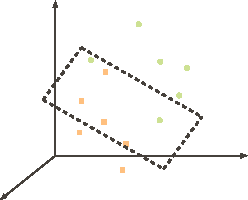
\includegraphics[width=\linewidth]{svm-hyperplane}
%            \begin{tikzpicture}[>=latex]
%
%                %\draw[help lines] (-1,-1) grid (5,4);
%                \draw[thick, ->] (0,0) -> (5.2,0);
%                \draw[thick, ->] (0,0) -> (0,4.2);
%                \draw[thick, ->] (0,0) -> (-1.5,-1.2);
%
%                \fill [hriSec2, opacity=0.5] (2.2,1.3) circle (2pt);
%                \fill [hriSec2, opacity=0.5] (2.5,0.4) circle (2pt);
%                \fill [hriSec2, opacity=0.5] (2.8,0.7) circle (2pt);
%                \fill [hriSec2, opacity=0.5] (3.8,1.7) circle (2pt);
%                \fill [hriSec2, opacity=0.5] (4.5,1.0) circle (2pt);
%                \fill [hriSec2, opacity=0.5] (4.1,2.4) circle (2pt);
%
%                \fill [hriSec3Comp, opacity=0.5] (2.3,3.2) rectangle +(3.5pt,3.5pt);
%                \fill [hriSec3Comp, opacity=0.5] (0.7,2.8) rectangle +(3.5pt,3.5pt);
%                \fill [hriSec3Comp, opacity=0.5] (1.7,3.8) rectangle +(3.5pt,3.5pt);
%                \fill [hriSec3Comp, opacity=0.5] (1.0,2.5) rectangle +(3.5pt,3.5pt);
%                \fill [hriSec3Comp, opacity=0.5] (2.2,2.5) rectangle +(3.5pt,3.5pt);
%                \fill [hriSec3Comp, opacity=0.5] (1.3,2.2) rectangle +(3.5pt,3.5pt);
%
%                \draw[dashed, ultra thick] (0,0.65) -- (4.9,3.45);
%                \draw[dashed, ultra thick] (0,0.65) -- (4.9,3.45);
%                \draw[dashed, ultra thick] (0,0.65) -- (4.9,3.45);
%                \draw[dashed, ultra thick] (0,0.65) -- (4.9,3.45);
%
%            \end{tikzpicture}
        }
        }
    \end{center}

\only<1>{

    A linear classifier for two categories (\textbf{binary classifier}) can be written as
    $f(\mathbf{x}) = \mathbf{w} \cdot \mathbf{x} + b$.

\begin{itemize}

    \item $\mathbf{w} \cdot \mathbf{x} = \sum_i w_i x_i$. This is called the
        scalar product or inner product. Can also be written as a matrix
        multiplication $\mathbf{w}^T\mathbf{x}$.
    \item $\mathbf{w}$ is a \textbf{weight vector}, tilting the line
    \item $\mathbf{x}$ is a data point (of dimension $n$)
    \item $b$ is a \textbf{bias}, lifting the line up along the $y$-axis
\end{itemize}

}
\only<2-3>{
    $\mathbf{w}$\bubblemark{weightvector} has to be calculated such that:
\[
f(\mathbf{x}) < 0 \Rightarrow \mathbf{x} \in \{\blacksquare\}
\]
\[
f(\mathbf{x}) > 0 \Rightarrow \mathbf{x} \in \{\circ\}
\]

\bubble<3>[115][0.8][4cm]{weightvector}{for kNNs, we have to carry along the training data; with a linear classifier, once $\mathbf{w}$ is found, we can discard the training data}
}



\only<4-5>{

    \begin{itemize}
        \item In 2D, the \textbf{discriminant} is a line
        \item In 3D, the discriminant is a plane
        \item In n-D\bubblemark{dimensions}, the discriminant is a hyperplane
    \end{itemize}

\bubble<5>[160][1][10cm]{dimensions}{the 'dimensions' are the \textbf{features} of our inputs, \eg for a human, the size, age, skin colour, gender...}
}

\end{frame}

\begin{frame}{Support vector classifier}

    \begin{center}
        \resizebox{0.3\linewidth}{!}{
            \begin{tikzpicture}[>=latex]

                \draw[thick, ->] (0,0) -> (5.2,0);
                \draw[thick, ->] (0,0) -> (0,4.2);

                \fill [hriSec2, opacity=0.5] (2.2,1.3) circle (2pt);
                \fill [hriSec2, opacity=0.5] (2.5,0.4) circle (2pt);
                \fill [hriSec2, opacity=0.5] (2.8,0.7) circle (2pt);
                \fill [hriSec2, opacity=0.5] (3.8,1.7) circle (2pt);
                \fill [hriSec2, opacity=0.5] (4.5,1.0) circle (2pt);
                \fill [hriSec2, opacity=0.5] (4.1,2.4) circle (2pt);

                \fill [hriSec3Comp, opacity=0.5] (2.3,3.2) rectangle +(3.5pt,3.5pt);
                \fill [hriSec3Comp, opacity=0.5] (0.7,2.8) rectangle +(3.5pt,3.5pt);
                \fill [hriSec3Comp, opacity=0.5] (1.7,3.8) rectangle +(3.5pt,3.5pt);
                \fill [hriSec3Comp, opacity=0.5] (1.0,2.5) rectangle +(3.5pt,3.5pt);
                \fill [hriSec3Comp, opacity=0.5] (2.2,2.5) rectangle +(3.5pt,3.5pt);
                \fill [hriSec3Comp, opacity=0.5] (1.3,2.2) rectangle +(3.5pt,3.5pt);


                \draw[red,opacity=0.5,line width=25pt] (0,0.65) -- (4.9,3.45);
                \draw[dashed, ultra thick] (0,0.65) -- (4.9,3.45);

                    \draw [red, thick] (2.25,2.55) circle (5pt);
                    \draw [red, thick] (4.1,2.4) circle (5pt);
                    \draw [red, thick] (2.2,1.3) circle (5pt);




            \end{tikzpicture}
        }
    \end{center}


In a SVM, we want to \textbf{maximise the margin} $M$. We can rewrite the linear
classifier.
    
If $\mathbf{w}^T\mathbf{x} + b \geq M$, then an observation belongs to
$\blacksquare$, for $\mathbf{w}^T\mathbf{x} + b \leq -M$, it belongs to
$\circ$.

\pause
A point $\mathbf{x}^\blacksquare$ that lies on the $\blacksquare$ class
    boundary line, \ie $\mathbf{w}^T\mathbf{x}^\blacksquare + b = M$, is
a \textbf{support vector}.


\end{frame}

\begin{frame}{Finding the optimal classifier}

The problem is to find the \textbf{optimal} values for $\mathbf{w}$ and
$b$.

The classifier needs to satisfy two conditions

\begin{itemize}

\item It needs to correctly classify the training data,
\item and needs the margin from the classifier to be as large as possible.
\end{itemize}

\pause

A \textbf{quadratic programming solver} is used to find the optimal
values for $\mathbf{w}$ and $b$.

{\footnotesize \href{http://www.robots.ox.ac.uk/~az/lectures/ml/lect2.pdf}{Oxford lecture on SVM} to learn more about the mathematical
    formulation and the \emph{perceptron algorithm}.}

\end{frame}

\begin{frame}{Transformation of data}

\begin{itemize}

    \item Unfortunately, \emph{all this still assumes that the data is linearly
        separable}. But what if it is not, and we are not prepared for a few
  misclassifications?
\item The solution is to \textbf{transform} the data: move data points in
  the n-D space until the training data is linearly separable again
\end{itemize}

    \begin{center}
        \includegraphics[width=0.8\linewidth]{svm-kernels}
    \end{center}
\end{frame}

\begin{frame}{Feature maps}

    \onslide<1-4>{
We can transform data points (= move them) or even add more dimensions using
a function $\theta(\mathbf{x}_i)$ from input $\mathbf{x}_i$. $\theta$ is a \textbf{feature
map}.
}

\only<1-2>{
Example:
    \onslide<2>{
    \[
        \theta(\mathbf{x}_i) = [\mathbf{x}_i, \mathbf{x}^2_i]
    \]
    }

\begin{center}
    \includegraphics<1>[width=0.8\linewidth]{svm-kernels-separation-0}
    \includegraphics<2>[width=0.8\linewidth]{svm-kernels-separation}
\end{center}


    \onslide<2>{
$\rightarrow$ now, linearly separable
}
}

\only<3-4>{
Example:
    \onslide<4>{
    \[
        \theta(<x_i, y_i>) = [x_i, y_i, x^2_i + y^2_i]
    \]
    }

\begin{center}
    \includegraphics<3>[width=0.7\linewidth]{svm-kernel-3d-0}
    \includegraphics<4>[width=0.7\linewidth]{svm-kernel-3d}
\end{center}

    \onslide<4>{
$\rightarrow$ now, linearly separable
    }
}
\only<5>{


If we know something about the structure of the data, then we might be able to identify
feature maps that would be effective.

Often however we do not have such domain knowledge.
}

\end{frame}

\begin{frame}{The kernel trick}

\[
        \theta: \mathbf{x} \rightarrow  \theta(\mathbf{x}), \mathbb{R}^d \rightarrow \mathbb{R}^D
\]

\[
    f(\mathbf{x}) = \mathbf{w}^T \theta(\mathbf{x}) + b
\]

\only<1>{
\begin{itemize}
    \item Simply map $\mathbf{x}$ to $\theta(\mathbf{x})$ where data is separable
    \item Solve for $\mathbf{w}$ in high dimensional space $\mathbb{R}^D$
    \item If $D >> d$ then there are many more parameters to learn for $\mathbf{w}$. Can this be avoided?
\end{itemize}
}

 \only<2>{
    \href{http://www.robots.ox.ac.uk/~az/lectures/ml/lect3.pdf}{It can be shown
    that} you do not actually need to calculate explicitely
    $\theta(\mathbf{x})$. Instead, you only need $\theta(\mathbf{x}_i)^T
    \theta(\mathbf{x}_j)$ (with $\mathbf{x}_i$ the training data) to compute
    $\mathbf{w}$.


    We call the \textbf{kernel function} $K(\mathbf{x}_i,\mathbf{x}_j) =
    \theta(\mathbf{x}_i)^T \theta(\mathbf{x}_j)$.  The SVM classifier can be
    learnt and applied with only $K$, and the complexity depends only on $N$
    (size of training data), not on $D$.  }

\end{frame}

\begin{frame}{Standard kernels}

\begin{itemize}

    \item \textbf{Polynomials} up to some degree $s$ in the
  elements $x_k$ of the input vector (\eg $x^3_3$ or $x_1 x_4$). This can be written as:

    \[
        K(x, y) = (1 + x^Ty)^s
    \]

\item \textbf{Sigmoid functions} of the $x_k$ with parameters $\kappa$ and $\delta$, and
  kernel:
    \[
        K(x, y) = tanh(\kappa x^T y - \delta)
    \]
\item \textbf{Radial basis function} expansions of the $x_k$ with parameter $\sigma$
  and kernel:
    \[
        K(x, y) = exp(- \frac{(x-y)^2}{2\sigma^2})
    \]

(a Gaussian kernel)

\end{itemize}

\end{frame}

\begin{frame}{Comparison of kernel functions}
    \begin{center}
        \includegraphics[width=\linewidth]{svm_comparison}
    \end{center}
\end{frame}

\begin{frame}[fragile]{Python implementation of Support Vector Machine}

\begin{onlyenv}<1>

\begin{pythoncode}
from sklearn import svm

C = 1.0  # SVM regularization parameter 
         # +- 'how acceptable are misclassification'
clf = svm.SVC(kernel='linear', C=C) # kernel='poly', 'rbf', 'sigmoid'...

clf.fit(data, categories)

predictions = clf.predict(inputs)
\end{pythoncode}

\end{onlyenv}

\begin{onlyenv}<2>
    Complete example, with our data:

\begin{columns}
    \begin{column}{0.4\linewidth}
\begin{pythoncode}
""" data.csv:
2.2,1.3,0 -> circles
3.2,2.3,0
...

2.3,3.2,1 -> squares
0.3,0.6,1
...

2.8,3.5,2 -> stars
3.2,2.6,2
...
"""
\end{pythoncode}
        
    \end{column}
    \begin{column}{0.6\linewidth}
\begin{pythoncode}
from numpy import genfromtxt
from sklearn import svm

csv = genfromtxt('data.csv', delimiter=',')
data = csv[:,:2]
categories = csv[:,2]


inputs = [ [3.5,3], [1.5,3], [1.8,1.9] ]

clf = svm.SVC(kernel='rbf',
              gamma = 0.7,
              C=1.0)
clf.fit(data, categories)

predictions = clf.predict(inputs)
print(predictions)

>>>  [2.  1.  0.]

\end{pythoncode}
    \end{column}
\end{columns}

\end{onlyenv}


\end{frame}

%\begin{frame}{Choosing the kernel}
%
%
%Choosing which kernel to use and the parameters in these kernels is a tricky
%    problem. While there reasoning based on the
%    \href{https://en.wikipedia.org/wiki/Vapnik-Chervonenkis_dimension}{Vapnik--Chernik
%    dimension} (a measure of the \emph{capacity} of your model) that can be
%    applied, most people just experiment with different values and find one that
%    works.
%
%\end{frame}

%\begin{frame}{Complexity of SVMs}
%
%
%SVMs do not work well on extremely large datasets, since the computations do
%    not scale well with the number of training examples, and so become
%    computationally very expensive.
%
%\begin{exampleblock}{Complexity}
%Training a SVM requires $O(m^3)$\bubblemark{bigo} operations and $O(m^2)$
%memory, with $m$ being the number of training samples.
%    
%For example with a NVidia GTX1080Ti ($\approx$350GFLOPs):
%
%    \begin{itemize}
%        \item 10,000 training samples $\rightarrow$ $10^{12}$ operations
%            $\rightarrow$ 2.9s ($10^{12}$ memory units).
%        \item 100,000 samples $\rightarrow$ 2900s
%        \item 1,000,000 samples $\rightarrow$ 2900000s $\equiv$ 33 days
%    \end{itemize}
%\end{exampleblock}
%
%\bubble<4>[190][1][6cm]{bigo}{For more information on ``big-O notation'',
%see \href{https://en.wikipedia.org/wiki/Time_complexity}{complexity of
%algorithms}}
%
%
%\end{frame}


\begin{frame}{Clustering vs classification}

\textbf{Clustering} is sometimes confused with \textbf{classification}.  (often
    because some algorithms have similar names,e.g. \emph{k-means clustering}
    and \emph{k-nearest neighbours}).

\textbf{Clustering} starts from unlabelled data points and tries to find
    $k$ clusters in the data $\rightarrow$ \textbf{unsupervised learning}.


$\rightarrow$ Used to find patterns in the data.

    \begin{center}
        \includegraphics[width=0.3\linewidth]{clustering-0}
        $\rightarrow$
        \includegraphics[width=0.3\linewidth]{clustering-1}
    \end{center}


    \textbf{Classification} starts from training data ($\rightarrow$
    \textbf{supervised learning}), and attempts to correctly classify an
    unknown observation.

\end{frame}

%%%%%%%%%%%%%%%%%%%%%%%%%%%%%%%%%%%%%%%%%%%%%%%%%%%%%%%%%%%%%%%%%%%%%%%
%%%%%%%%%%%%%%%%%%%%%%%%%%%%%%%%%%%%%%%%%%%%%%%%%%%%%%%%%%%%%%%%%%%%%%%
%%%%%%%%%%%%%%%%%%%%%%%%%%%%%%%%%%%%%%%%%%%%%%%%%%%%%%%%%%%%%%%%%%%%%%%


\section[Emotion classifier]{Let's build our own emotion classifier from scratch}

\begin{frame}{Shopping list}

    \begin{center}
        {\bf What do we need?}
    \end{center}

    \pause

    \begin{itemize}
        \item<+-> a dataset of labelled faces
        \item<+-> some pre-processing to normalise the faces
        \item<+-> features to extract
        \item<+-> a classifier
    \end{itemize}
\end{frame}

\imageframe[color=black]{emotions/google-emotions-query}
\imageframe[color=black]{emotions/emotions_dataset}
\imageframe[color=black]{emotions/emotions_dataset_aligned}


\begin{frame}{Features: Facial Action Units}

    \newcommand{\au}[1]{
        \includegraphics[width=2cm]{emotions/au/au-0####1.jpg}
    }

    \begin{columns}
        \begin{column}{0.5\linewidth}
            \begin{center}

                \scriptsize
                \begin{tabular}{@{}p{0.3cm}p{2.5cm}p{2cm}@{}}
                    \toprule
                    \textbf{AU} & \textbf{Description} & \textbf{Example image} \\
                    \midrule
                    \only<1>{
                        \textbf{1}  & Inner Brow Raiser    &  \au{01} \\
                    \textbf{2}  & Outer Brow Raiser    &  \au{02} \\
                    \textbf{4}  & Brow Lowerer         &  \au{04} \\
                    \textbf{5}  & Upper Lid Raiser     &  \au{05} \\
                    \textbf{6}  & Cheek Raiser         &  \au{06} \\
                    \bottomrule
                }
                    \only<2>{
                        \textbf{15} & Lip Corner Depressor &  \au{15} \\
                    \textbf{17} & Chin Raiser          &  \au{17} \\
                    \textbf{20} & Lip stretcher        &  \au{20} \\
                    \textbf{23} & Lip Tightener        &  \au{23} \\
                    \bottomrule
                }
                \end{tabular}
            \end{center}

        \end{column}
        \begin{column}{0.5\linewidth}
            \begin{center}

                \scriptsize
                \begin{tabular}{@{}p{0.3cm}p{2cm}p{2cm}@{}}
                    \toprule
                    \textbf{AU} & \textbf{Description} & \textbf{Example image} \\
                    \midrule
                    \only<1>{
                        \textbf{7}  & Lid Tightener        &  \au{07} \\
                    \textbf{9}  & Nose Wrinkler        &  \au{09} \\
                    \textbf{10} & Upper Lip Raiser     &  \au{10} \\
                    \textbf{12} & Lip Corner Puller    &  \au{12} \\
                    \bottomrule
                }
                    \only<2>{
                        \textbf{14} & Dimpler              &  \au{14} \\
                    \textbf{25} & Lips part            &  \au{25} \\
                    \textbf{26} & Jaw Drop             &  \au{26} \\
                    \textbf{45} & Blink                &          \\
                    \bottomrule
                }
                \end{tabular}
            \end{center}
        \end{column}
    \end{columns}

\end{frame}

\begin{frame}{OpenFace Action Units}
    \begin{center}
        OpenFace is an open-source library that recognises 17 action units
        (amongst many other things).

        \href{https://github.com/TadasBaltrusaitis/OpenFace}{github.com/TadasBaltrusaitis/OpenFace}
        \vspace{2em}

        \includegraphics[width=0.9\linewidth]{emotions/au-openface}

        \scriptsize
        (not to be confused with this other \href{https://github.com/cmusatyalab/openface}{CMU OpenFace})
    \end{center}
\end{frame}




\imageframe[color=black]{emotions/emotion-dataset-csv}

\begin{frame}{Our tiny 'emotions' dataset}
    \begin{itemize}
        \item A couple of \href{https://www.google.co.uk/search?q=human+face+happiness&tbm=isch&source=lnt&tbs=itp:face}{Google queries}
        \item a bit of manual filtering
        \item 558 faces, between 70 and 130 per emotion
        \item split into 2 datasets: a {\bf training} dataset (50 face per
            emotion) and a {\bf testing} dataset
        \item for each face, OpenFace pre-processing to:
            \begin{itemize}
                \item extract facial landmarks
                \item normalise and mask out the faces
                \item extract action units
            \end{itemize}
    \end{itemize}

    The dataset is available for you to play with on the lecture's
    \href{https://github.com/severin-lemaignan/lecture-hri-emotions}{GitHub repo}.
\end{frame}


\begin{frame}[fragile]{Classification results, Action Units}
    

    \begin{center}
        {\bf $n$ = 17 dimensions (i.e., 17 action units)}
    \end{center}

    \begin{columns}
        \begin{column}{0.4\linewidth}
    {\bf kNN}:
    \begin{itemize}
        \item k=1: 46.9\%
        \item k=2: 42.2\%
        \item k=4: 50.8\%
        \item k=6: 46.1\%
        \item k=9: 52.3\%
    \end{itemize}

    {\bf SVM}:

    \begin{itemize}
        \item kernel: rbf: 48.8\%
        \item kernel: linear: 52.3\%
        \item kernel: poly: 38.0\%
    \end{itemize}

    \onslide<2>{
        \textbf{Chance}: 16.7\%
    }

        \end{column}
        \begin{column}{0.6\linewidth}
            \begin{pythoncode}
from numpy import genfromtxt
from sklearn import neighbors, svm

csv_train = genfromtxt('training.csv')
training = csv_train[:,1:-1]
training_categories = csv_train[:,0]

csv_test = genfromtxt('testing.csv')
testing = csv_test[:,1:-1]
testing_categories = csv_test[:,0]

clf = neighbors.KNeighborsClassifier(k)
clf.fit(training, training_categories)
knns_predictions = clf.predict(testing)

clf = svm.SVC(kernel=kernel)
clf.fit(training, training_categories)
svm_predictions = clf.predict(testing)

            \end{pythoncode}
        \end{column}
    \end{columns}

\end{frame}

\imageframe[color=black,caption=Natural emotions are much harder]{emotions/natural-emotions-hulot}


\begin{frame}{Multi-modal social processing}

    We can usually improve social signal processing by \textbf{combining several
    modalities}.

    \begin{center}
        \audio{figs/prosody/media1.mp4}\hspace{0.3em}
        \audio{figs/prosody/media2.mp4}\hspace{0.3em}
        \audio{figs/prosody/media3.mp4}\hspace{0.3em}
        \audio{figs/prosody/media4.mp4}\hspace{0.3em}
        \audio{figs/prosody/media5.mp4}
    \end{center}
    \source{http://emodb.bilderbar.info/start.html}{Berlin Database of
    Emotional Speech}

    \only<2>{
        „Sie haben es gerade hochgetragen und jetzt gehen sie wieder runter``
    (They just carried it upstairs and now they are going down again).



    Which emotion do you recognise?


    \textbf{Anger} -- \textbf{Boredom} -- \textbf{Disgust} -- \textbf{Anxiety/Fear} -- \textbf{Happiness} --
    \textbf{Sadness} --  \textbf{Neutral}
}

    \only<3>{
    \textbf{Prosody} is an important \emph{non-verbal} social signal.

        Humans recognise emotions from prosody with approx. 80\% accuracy
    (\textit{caveat: this is for speech spoken by actors in a recording studio})

}


\end{frame}



\begin{frame}{We've barely scratched the surface!}

Social signal processing is extracting relevant information from the
social environment.

Some work relatively well

\begin{itemize}

\item Face \textbf{detection}, voice activity detection, gender
  classification, \ldots{}
\end{itemize}

Some work, but need improvement

\begin{itemize}

\item Gaze detection, basic emotion recognition, face \textbf{recognition},
  speech recognition, \ldots{}
\end{itemize}

But still many open problems remaining

\begin{itemize}

\item Complex real-word affect and emotion recognition (e.g.~embarrassment,
  pride).
\item Speech recognition for atypical speakers (children, elderly),
  multi-party interaction, \ldots{}
\end{itemize}

\end{frame}

\miniframesoff

\begin{frame}{}
    \begin{center}
        \Large
        That's all for today, folks!\\[2em]
        \normalsize
        Questions:\\
        \url{severin.lemaignan@brl.ac.uk} \\[1em]

        Slides:\\ \href{https://github.com/severin-lemaignan/lecture-social-signal-processing}{\small github.com/severin-lemaignan/lecture-social-signal-processing}

    \end{center}
\end{frame}


\begin{frame}{Classification of auditory signals}

    Raw signals will in most cases require pre-processing to extract
features.

The raw social signal (audio or video) requires pre-processing\bubblemark{preprocessing} to
extract between 10 and over a 1000 \textbf{features}.

\begin{itemize}

    \item A raw signals contains too much data, and cannot be fed to the
      classifier immediately.

        \begin{center}
            \includegraphics[width=0.5\linewidth]{rawaudio}
        \end{center}

    \item Pre-processing extracts feature data which is relevant for the
  information which we are after (pitch, volume/energy, duration,
  formant frequencies, \ldots{})
    \item These features then form the input for the classifier.
\end{itemize}

    {\footnotesize
For more information see, for example, Liang et al. (2005)
\href{http://ieeexplore.ieee.org/xpls/icp.jsp?arnumber=1571239}{Feature
analysis and extraction for audio automatic classification}, Systems,
Man and Cybernetics, 2005 IEEE International Conference on.
    }

\bubble<2>[50][0.7][5cm]{preprocessing}{An exception to this are Convolutional Neural
    Networks, which can deal with unprocessed data}

\end{frame}

\begin{frame}{Example: recognising gender from speech}

Can we automatically recognise someone's gender from speech?

3,168 recorded voice samples, collected from male and female speakers.

\begin{itemize}

\item Examples from the database: male (US), female (US), male (Scotish)
\end{itemize}

    \begin{center}
    \audio{figs/male-us.mp4}\hspace{0.3em}
    \audio{figs/male-scottish.mp4}\hspace{0.3em}
    \audio{figs/female-us.mp4}
    \end{center}


The voice samples are pre-processed by acoustic analysis in R using the
{\tt seewave}, {\tt warbleR} and {\tt tuneR} packages, with an analysed frequency range of
0hz-280Hz (fundamental frequency of human speech).


\source{https://www.kaggle.com/primaryobjects/voicegender}{data and more information}


\end{frame}

\begin{frame}{The 20 features used for gender classification}

    \only<1>{
\begin{itemize}

\item \textbf{meanfreq}: mean frequency (in kHz)
\item \textbf{sd}: standard deviation of frequency
\item \textbf{median}: median frequency (in kHz)
\item \textbf{Q25}: first quantile (in kHz)
\item \textbf{Q75}: third quantile (in kHz)
\item \textbf{IQR}: interquantile range (in kHz)
\item \textbf{skew}: skewness (see note in specprop description)
\item \textbf{kurt}: kurtosis (see note in specprop description)
\item \textbf{sp.ent}: spectral entropy
\item \textbf{sfm}: spectral flatness
\item \textbf{mode}: mode frequency
\item \textbf{centroid}: frequency centroid (see specprop)
\item \textbf{peakf}: peak frequency (frequency with highest energy)
\item \textbf{meanfun}: average of fundamental frequency measured across
  acoustic signal
\end{itemize}
}
    \only<2>{
\begin{itemize}

\item \textbf{minfun}: minimum fundamental frequency measured across
  acoustic signal
\item \textbf{maxfun}: maximum fundamental frequency measured across
  acoustic signal
\item \textbf{meandom}: average of dominant frequency measured across
  acoustic signal
\item \textbf{mindom}: minimum of dominant frequency measured across
  acoustic signal
\item \textbf{maxdom}: maximum of dominant frequency measured across
  acoustic signal
\item \textbf{dfrange}: range of dominant frequency measured across acoustic
  signal
\item \textbf{modindx}: modulation index. Calculated as the accumulated
  absolute difference between adjacent measurements of fundamental
  frequencies divided by the frequency range
\end{itemize}
}

\end{frame}

\begin{frame}{Example: recognising gender from speech}

    \begin{center}
        \includegraphics[width=\linewidth]{vector-gender-voice}
    \end{center}
\end{frame}

\begin{frame}{Example: recognising gender from speech}

Performance

\begin{itemize}

\item kNN (k = 7): 97.8\% classified correctly.
\item SVM: 97.5\% classified correctly.
\end{itemize}

Recognising gender from speech is easy and robust.

All classification algorithms can deal with this problem.

\end{frame}


\end{document}
